\documentclass[aspectratio=169]{beamer}

\usetheme{UiO}

\usepackage{array}
\usepackage{emoji}
\usepackage{pgfplots}
\usepackage{pgfplotstable}

\usetikzlibrary{arrows.meta}

\title{En introduksjon til kunstig intelligens}
\subtitle{Og dets rolle i medisinsk forskning}
\author{Esten H. Leonardsen}
\date{\today}

\def\systemfont{\footnotesize}

\def\vsep{0.5}
\def\hsep{0.65}
\def\edgeopacity{0.5}

\newcommand{\neuron}[3][uiogreen]{
    \node[circle, draw=black, fill=#1, minimum size=0.3cm] (#2) at #3 {};
}

\pgfplotsset{
    discard if not/.style 2 args={
        x filter/.code={
            \edef\tempa{\thisrow{#1}}
            \edef\tempb{#2}
            \ifx\tempa\tempb
            \else
                \def\pgfmathresult{inf}
            \fi
        }
    }
}
\pgfplotsset{
    discard if/.style 2 args={
        x filter/.code={
            \edef\tempa{\thisrow{#1}}
            \edef\tempb{#2}
            \ifx\def\pgfmathresult{inf}
            \else
                \tempa\tempb
            \fi
        }
    }
}


\begin{document}
	\begin{frame}
	 	\titlepage
	\end{frame}

    \newcommand{\mriside}[4]{
    \def\mridepth{0.75}

    \node[inner sep=0pt] (input) at (#1, #2) {
        \includegraphics[height=#3, width=#3]{#4}
    };

    \draw[fill=black] (input.north west) --
        ($ (input.north west) + (0.5 * \mridepth, 0.5 * \mridepth) $) --
        ($ (input.north east) + (0.5 * \mridepth, 0.5 * \mridepth) $) --
        (input.north east) -- cycle;
    \draw[fill=black] (input.north east) --
        ($ (input.north east) + (0.5 * \mridepth, 0.5 * \mridepth) $) --
        ($ (input.south east) + (0.5 * \mridepth, 0.5 * \mridepth) $) --
        (input.south east) -- cycle;
    \draw[] (input.north west) --
        ($ (input.north west) - (0.5 * \mridepth, 0.5 * \mridepth) $) --
        ($ (input.south west) - (0.5 * \mridepth, 0.5 * \mridepth) $) --
        (input.south west) -- cycle;
    \draw[] (input.north east) --
        ($ (input.north east) - (0.5 * \mridepth, 0.5 * \mridepth) $) --
        ($ (input.south east) - (0.5 * \mridepth, 0.5 * \mridepth) $) --
        (input.south east) -- cycle;
    \draw[] ($ (input.north west) - (0.5 * \mridepth, 0.5 * \mridepth) $) --
        ($ (input.north east) - (0.5 * \mridepth, 0.5 * \mridepth) $);
    \draw[] ($ (input.south west) - (0.5 * \mridepth, 0.5 * \mridepth) $) --
        ($ (input.south east) - (0.5 * \mridepth, 0.5 * \mridepth) $);
}


\newcommand{\inputside}[3]{
    \mriside{#1}{#2}{#3}{data/mri_sagittal.png}
}

\newcommand{\heatmapside}[3]{
    \mriside{#1}{#2}{#3}{data/combined_sagittal.png}
}

\newcommand{\convside}[6]{
    \def\sidex{#1}
    \def\sidey{#2}
    \def\sidewidth{#3}
    \def\sideheight{#4}
    \def\sidefillcolour{#5}
    \def\sidename{#6}

    \node[
        fill=\sidefillcolour,
        inner sep=0pt,
        outer sep=0pt,
        minimum width=\sidewidth,
        minimum height=\sideheight,
        draw=black
    ] (\sidename) at (\sidex, \sidey) {};
}

\newcommand{\convtop}[4]{
    \def\topbase{#1}
    \def\topwidth{#2}
    \def\topheight{#3}
    \def\topfillcolour{#4}

    \draw[fill=\topfillcolour,draw=black] #1 --
        ($ #1 + (#3, #3) $) --
        ($ #1 + (#3+#2, #3) $) --
        ($ #1 + (#2, 0) $);
}

\newcommand{\convfront}[3]{
    \def\frontbase{#1}
    \def\frontsize{#2}
    \def\frontfillcolour{#3}

    \draw[black, fill=\frontfillcolour] #1 --
        ($ #1 + (1*#2, 1*#2) $) --
        ($ #1 + (1*#2, 1*#2 - 2*#2) $) --
        ($ #1 + (0, -2*#2) $);
}

\newcommand{\convchannel}[7]{
    \def\channelx{#1}
    \def\channely{#2}
    \def\channelnodedepth{#3}
    \def\channelnodesize{#4}
    \def\channelnodecount{#5}
    \def\channelcolour{#6}
    \def\includefront{#7}

    \def\huemin{20}
    \def\huemax{80}

    \pgfmathsetmacro{\iterations}{#5-1}
    \foreach \i in {0,...,\iterations} {
        \pgfmathsetmacro{\hue}{int(random(\huemin, \huemax))}
        \convside{#1}{#2+\i*-#4}{#3 cm}{#4 cm}{#6!\hue}{n\i0}

        \foreach \j in {0,...,\iterations} {
            \pgfmathsetmacro{\innerhue}{int(random(\huemin, \huemax))}
            \ifnum\j=0
                \pgfmathsetmacro{\innerhue}{\hue}
            \fi

            \ifnum\includefront=1
                \convfront{($ (n00.north east) + (0.5*\j*#4, 0.5*\j*#4 - \i*#4) $)}{0.5*#4}{#6!\innerhue}
            \fi

            \ifnum\i=0
                \convtop{($ (n\i0.north west) + (0.5*\j*#4, 0.5*\j*#4) $)}{#3}{0.5*#4}{#6!\innerhue}
            \fi
        }
    }
}
\newcommand{\lrpchannel}[6]{
    \def\channelx{#1}
    \def\channely{#2}
    \def\channelnodedepth{#3}
    \def\channelnodesize{#4}
    \def\channelnodecount{#5}
    \def\includefront{#6}

    \colorlet{bgcolour}{black!85}

    \pgfmathsetmacro{\iterations}{#5-1}
    \foreach \i in {0,...,\iterations} {
        \pgfmathsetmacro{\hue}{int(random(-150, 100))}
        \colorlet{fillcolour}{bgcolour}

        \colorlet{lrpcolour}{red}
        \pgfmathsetmacro{\coinflip}{int(random(0, 1))}

        \ifnum\coinflip=1
            \colorlet{lrpcolour}{blue}
        \fi

        \ifnum\hue>0
            \colorlet{fillcolour}{lrpcolour!\hue!bgcolour}
        \fi

        \convside{#1}{#2+\i*-#4}{#3 cm}{#4 cm}{fillcolour}{n\i0}

        \foreach \j in {0,...,\iterations} {
            \pgfmathsetmacro{\innerhue}{int(random(-150, 100))}
            \colorlet{innerfillcolour}{bgcolour}

            \ifnum\innerhue>0
                \colorlet{innerfillcolour}{lrpcolour!\innerhue!bgcolour}
            \fi

            \ifnum\j=0
                \colorlet{innerfillcolour}{fillcolour}
            \fi

            \ifnum\includefront=1
                \convfront{($ (n00.north east) + (0.5*\j*#4, 0.5*\j*#4 - \i*#4) $)}{0.5*#4}{innerfillcolour}
            \fi

            \ifnum\i=0
                \convtop{($ (n\i0.north west) + (0.5*\j*#4, 0.5*\j*#4) $)}{#3}{0.5*#4}{innerfillcolour}
            \fi
        }
    }
}


\newcommand{\convlayer}[7]{
    \def\layerx{#1}
    \def\layery{#2}
    \def\layernodedepth{#3}
    \def\layernodesize{#4}
    \def\layernodecount{#5}
    \def\layerdepth{#6}
    \def\layercolour{#7}

    \pgfmathsetmacro{\layeriterations}{\layerdepth-1}
    \foreach \i in {0,...,\layeriterations}{
        \pgfmathsetmacro{\x}{\layerx + \i * \layernodedepth}
        \pgfmathsetmacro{\islast}{\i == \layeriterations ? 1 : 0}
        \convchannel{\x}{\layery}{\layernodedepth}{\layernodesize}{\layernodecount}{\layercolour}{\islast}
    }
}
\newcommand{\lrplayer}[6]{
    \def\layerx{#1}
    \def\layery{#2}
    \def\layernodedepth{#3}
    \def\layernodesize{#4}
    \def\layernodecount{#5}
    \def\layerdepth{#6}

    \pgfmathsetmacro{\layeriterations}{\layerdepth-1}
    \foreach \i in {0,...,\layeriterations}{
        \pgfmathsetmacro{\x}{\layerx + \i * \layernodedepth}
        \pgfmathsetmacro{\islast}{\i == \layeriterations ? 1 : 0}
        \lrpchannel{\x}{\layery}{\layernodedepth}{\layernodesize}{\layernodecount}{\islast}
    }
}

\newcommand{\modelarrow}[5]{
    \begin{scope}[transparency group, opacity=0.5]
        \draw[-stealth, line width=2pt, #3] #1 to [in=#4, out=#5] #2;
    \end{scope}
}
\newcommand{\cnnarrow}[3]{
    \modelarrow{#1}{#2}{#3}{180}{0}
}
\newcommand{\lrparrow}[3]{
    \modelarrow{#1}{#2}{#3}{0}{180}
}

\newcommand{\cnn}[6]{
    \def\xmin{#1}
    \def\ymin{#2}
    \def\nodedepth{#3}
    \def\nodesize{#4}
    \def\modelcolour{#5}
    \def\annotate{#6}

    \convlayer{#1 - 0.06 + 0.4}{#2 + 2.5 * #4}{#3}{#4}{12}{3}{\modelcolour}
    \cnnarrow{(#1 + 1.04, #2)}{(#1+2.2, #2)}{black}

    \convlayer{#1 + 1.44 + 0.4}{#2 + 1.5 * #4}{#3}{#4}{8}{5}{\modelcolour}
    \cnnarrow{(#1 + 2.59, #2)}{(#1+3.5, #2)}{black}

    \convlayer{#1 + 2.77 + 0.4}{#2 + 0.5 * #4}{#3}{#4}{4}{7}{\modelcolour}
    \cnnarrow{(#1 + 3.98, #2)}{(#1+5, #2)}{black}

    \convlayer{#1 + 3.93 + 0.4}{#2 + 0}{#3}{#4}{2}{9}{\modelcolour}

    \draw[thick, dashed] (#1 + 0.22, #2 + 1.43) --
                        (#1 + 5.4, #2 + 1.43) --
                        (#1 + 5.4, #2 - 1.42) --
                        (#1 + 0.22, #2 - 1.42) -- cycle;
    \node[anchor=south, text depth=0, font=\footnotesize\selectfont] at (#1 + 2.675, #2 + 1.43) {
        \textbf{Convolutional neural network}
    };
}
\newcommand{\lrp}[4]{
    \def\xmin{#1}
    \def\ymin{#2}
    \def\nodedepth{#3}
    \def\nodesize{#4}

    \lrplayer{#1 - 0.06 + 0.4}{#2 + 2.5 * #4}{#3}{#4}{12}{3}{black}
    \lrparrow{(#1+2.2, #2)}{(#1 + 1.04, #2)}{black}

    \lrplayer{#1 + 1.44 + 0.4}{#2 + 1.5 * #4}{#3}{#4}{8}{5}{black}
    \lrparrow{(#1+3.5, #2)}{(#1 + 2.59, #2)}{black}

    \lrplayer{#1 + 2.77 + 0.4}{#2 + 0.5 * #4}{#3}{#4}{4}{7}{black}
    \lrparrow{(#1+5, #2)}{(#1 + 3.98, #2)}{black}

    \lrplayer{#1 + 3.93 + 0.4}{#2 + 0}{#3}{#4}{2}{9}{black}

    \draw[thick, dashed] (#1 + 0.22, #2 + 1.43) --
                        (#1 + 5.4, #2 + 1.43) --
                        (#1 + 5.4, #2 - 1.42) --
                        (#1 + 0.22, #2 - 1.42) -- cycle;
    \node[anchor=south, text depth=0, font=\footnotesize\selectfont] at (#1 + 2.675, #2 + 1.43) {
        \textbf{Convolutional Neural Network}
    };
}
    %
\begin{frame}{What is artificial intelligence?}
    \begin{tikzpicture}
        \node[] at (-7, -3.25) {};
        \node[] at (7, 3.25) {};

        \only<1>{
            \node[anchor=west, inner sep=0pt, draw=black, label=below:\tiny{ChatGPT}] at (-7, 0) {
                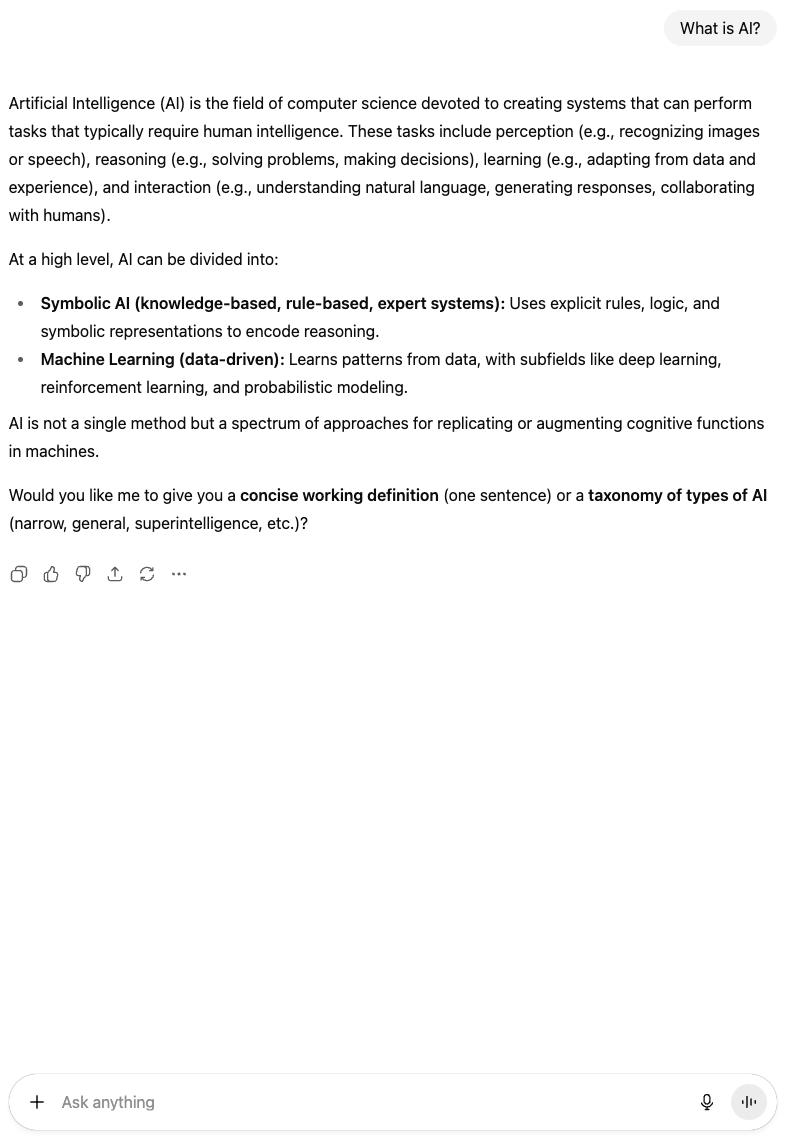
\includegraphics[width=4.1cm]{data/chatgpt.png}
            };
            \node[inner sep=0pt, draw=black, label=below:\tiny{Spot}] at (-0.5, 1.5) {
                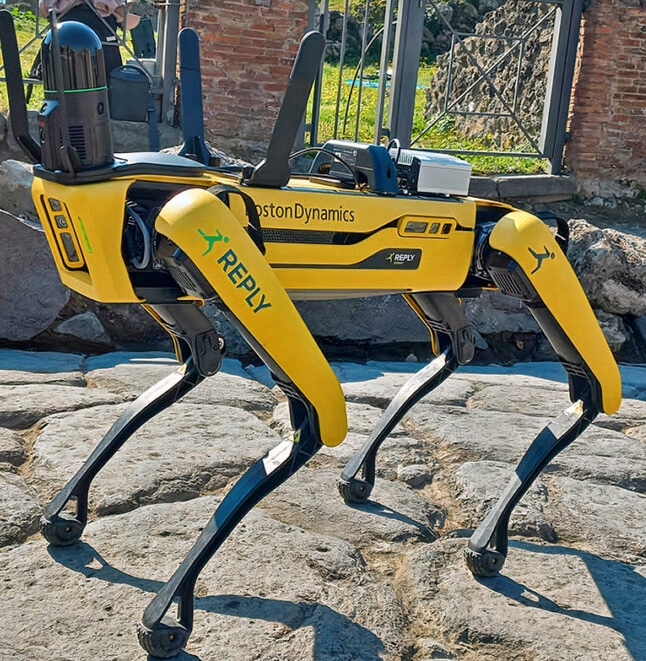
\includegraphics[width=2.5cm]{data/spot.jpg}
            };
            \node[inner sep=0pt, draw=black, label=below:\tiny{Sophia}] at (2.7, 1.9) {
                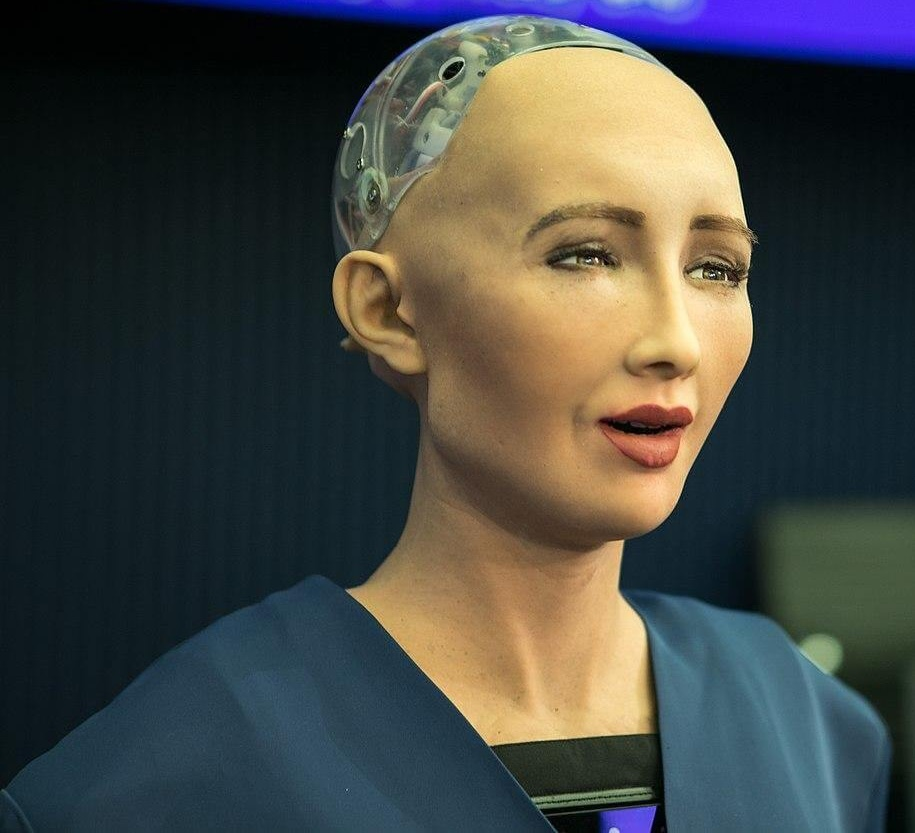
\includegraphics[width=2.5cm]{data/sophia.jpg}
            };
            \node[inner sep=0pt, draw=black, label=below:\tiny{AlphaFold}] at (1, -1.8) {
                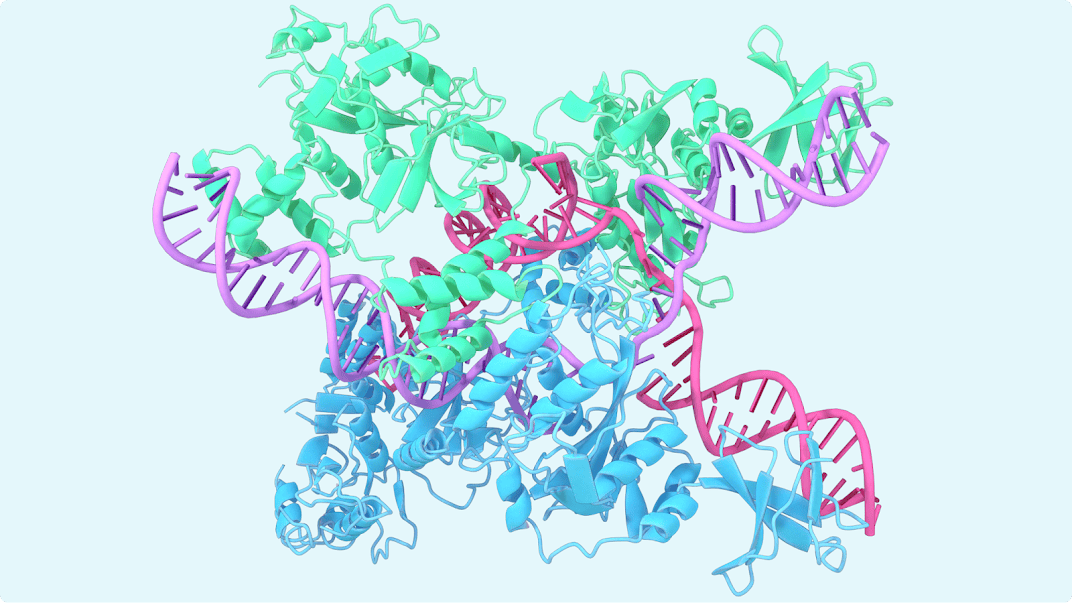
\includegraphics[width=3cm]{data/alphafold.png}
            };
            \node[inner sep=0pt, draw=black, label=below:\tiny{AlphaZero}] at (4.5, -1.1) {
                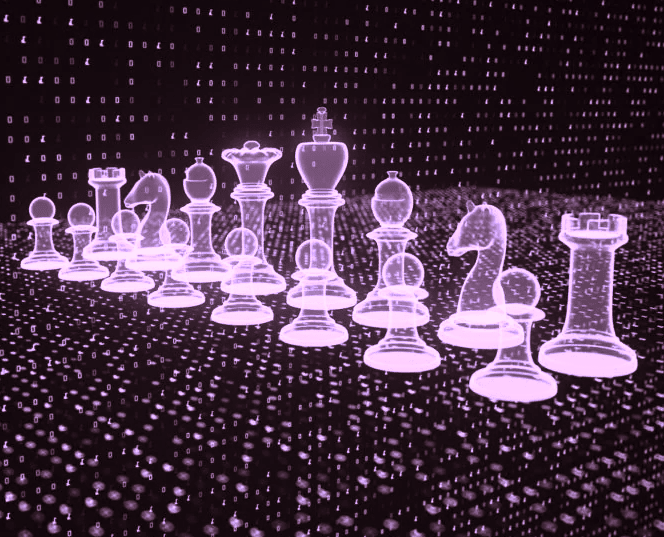
\includegraphics[width=2.7cm]{data/chess.png}
            };
        }

        \only<2>{
            \node[circle, fill=uioblue!80, minimum size=6cm, anchor=north] (ai) at (-4, 3.25) {};
            \node[white, anchor=north, align=center, font=\small\bfseries\linespread{0.9}\selectfont] at ($ (ai.north) - (0, 0.1) $) {Artificial\\intelligence};
            \node[align=flush left, anchor=north west, text width=7.2cm, font=\small\linespread{0.95}\selectfont] (def1) at (-0.5, 3.25) {
                \textbf{Artificial intelligence}\\
                The field of study producing technology that solves tasks requiring some form of intelligence
            };
            \node[circle, fill=uioblue!50!uiored!80, anchor=south, minimum size=4.1cm] (ml) at ($ (ai.south) + (0, 0.05) $) {};
            \node[white, anchor=north, align=center, font=\small\bfseries\linespread{0.9}\selectfont] at ($ (ml.north) - (0, 0.1) $) {Machine\\learning};
            \node[align=center, font=\small\linespread{0.9}\selectfont, text=white] at ($ (ai.north) + (1.3, -1.5) $) {Rule-based\\systems};
            \node[align=flush left, anchor=north west, text width=7.2cm, font=\small\linespread{0.95}\selectfont] (def2) at (def1.south west) {
                \textbf{Machine learning}\\
                A set of techniques to solve problems by allowing machines to find patterns in training data
            };
            \node[circle, fill=uiored!80, anchor=south, minimum size=3cm] (dl) at ($ (ml.south) + (0, 0.06) $) {};
            \node[white, anchor=north, align=center, font=\small\bfseries\linespread{0.9}\selectfont] at ($ (dl.north) - (0, 0.1) $) {Deep\\learning};
            \node[align=flush left, anchor=north west, text width=7.2cm, font=\small\linespread{0.95}\selectfont] (def3) at (def2.south west) {
                \textbf{Deep learning}\\
                    Machine learning approaches that rely on artificial neural networks
                };

        }
    \end{tikzpicture}
\end{frame}

\newcommand{\brainsize}[1]{
    \begin{tikzpicture}
        \begin{axis}[
            width=8cm,
            height=3.8cm,
            xlabel=\footnotesize{Age},
            ylabel=\footnotesize{Brain size},
            xmajorticks=false,
            ymajorticks=false,
            axis lines=left,
            xmin=2,
            xmax=13,
            ymin=935,
            ymax=1600
        ]
            \addplot[
                only marks,
                uioblue,
                opacity=0.5
            ] table [
                col sep=comma,
                x=x,
                y=y
            ] {data/brainsize.csv};

            \ifnum#1=1
                \addplot[
                    samples=100,
                    domain=2:15,
                    very thick,
                    uioblue
                ] {
                    1064.062904437416+x*36.95459273
                };
            \fi
            \ifnum#1=2
                \addplot[
                    samples=100,
                    domain=2:15,
                    very thick,
                    uioblue
                ] {
                    400+1100*(1-e^(-x/3))
                };
            \fi
        \end{axis}
    \end{tikzpicture}
}

\begin{frame}{Why do we use artificial neural networks?}
    \begin{tikzpicture}
        \node[] at (-7, -3.25) {};
        \node[] at (7, 3.25) {};

        \visible<1-3>{
            \node[anchor=east] (input) at (-3, 1.25) {$\text{input}$};
            \node[anchor=west] (output) at (3, 1.25) {$\text{output}$};
        }
        \visible<2>{
            \node[] at (-0.25, -1.85) {
                \brainsize{0}
            };
        }
        \visible<3>{
            \node[] at (-0.25, -1.85) {
                \brainsize{2}
            };
        }
        \visible<4>{
            \node[anchor=east, inner sep=0pt, draw=black] (input) at (-3, 1.25) {
                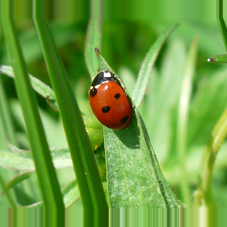
\includegraphics[width=2.5cm]{data/ladybug.png}
            };
            \node[anchor=west] (output) at (3, 1.25) {$\text{ladybug}$};
        }
        \visible<5>{
            \node[anchor=east, inner sep=0pt] (input1) at (-4, 2.75) {
                {\Huge{\emoji{spiral-notepad}}}
            };
            \node[anchor=east, inner sep=0pt, draw=black] (input2) at (-4, 1.25) {
                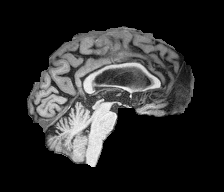
\includegraphics[width=1.5cm]{data/mri_sagittal.png}
            };
            \node[anchor=east, inner sep=0pt] (input3) at (-4, -0.25) {
                {\Huge{\emoji{microscope}}}
            };
            \node[anchor=west, align=left] (output) at (3, 1.25) {
                Clinical\\
                prediction
            };
        }

        \node[fill=gray!80, minimum width=4cm, minimum height=2.9cm, rounded corners=0.1cm, text=white, draw=black, font=\systemfont, anchor=south, text depth=2.4cm] (model) at (0, 0) {
            Artificial neural network
        };
        \only<1-4>{
            \draw[-stealth] (input.east) -- ($ (model.south west) + (0, 1.25) $);
        }
        \draw[-stealth] ($ (model.south east) + (0, 1.25) $) -- (output);
        \neuron{n00}{($ (model.south) + (0, 1.25) + (-2*\hsep, -2*\vsep) $)}
        \neuron{n01}{($ (n00) + (0, \vsep) $)}
        \neuron{n02}{($ (n00) + (0, 2*\vsep) $)}
        \neuron{n03}{($ (n00) + (0, 3*\vsep) $)}
        \neuron{n04}{($ (n00) + (0, 4*\vsep) $)}

        \neuron{n10}{($ (n00) + (\hsep, 0.5*\vsep) $)}
        \neuron{n11}{($ (n00) + (\hsep, 1.5*\vsep) $)}
        \neuron{n12}{($ (n00) + (\hsep, 2.5*\vsep) $)}
        \neuron{n13}{($ (n00) + (\hsep, 3.5*\vsep) $)}

        \neuron{n20}{($ (n00) + (2*\hsep, \vsep) $)}
        \neuron{n21}{($ (n00) + (2*\hsep, 2*\vsep) $)}
        \neuron{n22}{($ (n00) + (2*\hsep, 3*\vsep) $)}

        \neuron{n30}{($ (n00) + (3*\hsep, 1.5*\vsep) $)}
        \neuron{n31}{($ (n00) + (3*\hsep, 2.5*\vsep) $)}

        \neuron{n40}{($ (n00) + (4*\hsep, 2*\vsep) $)}

        \foreach \j in {0,...,4} {
            \draw[black, opacity=\edgeopacity] ($ (model.west) - (0, 0.2175) $) -- (n0\j);
        }

        \foreach \j in {0,...,4} {
            \foreach \k in {0,...,3} {
                \draw[black, opacity=\edgeopacity] (n0\j) -- (n1\k);
            }
        }
        \foreach \j in {0,...,3} {
            \foreach \k in {0,...,2} {
                \draw[black, opacity=\edgeopacity] (n1\j) -- (n2\k);
            }
        }
        \foreach \j in {0,...,2} {
            \foreach \k in {0,...,1} {
                \draw[black, opacity=\edgeopacity] (n2\j) -- (n3\k);
            }
        }
        \draw[black, opacity=\edgeopacity] (n30) -- (n40);
        \draw[black, opacity=\edgeopacity] (n31) -- (n40);
        \draw[black, opacity=\edgeopacity] (n40) -- ($ (model.south east) + (0, 1.25) $);

        \only<1>{
            \node[circle, draw=black, fill=uiogreen, minimum size=0.5cm] (neuron) at ($ (model.south) - (0, 1.5) $) {};

            \node[anchor=east, font=\scriptsize] (x1) at ($ (neuron) - (0.75, -0.5) $) {$\text{input}_1$};
            \node[anchor=east, font=\scriptsize] (x2) at ($ (neuron) - (0.75, 0) $) {$\text{input}_2$};
            \node[anchor=east, font=\scriptsize] (x3) at ($ (neuron) - (0.75, 0.5) $) {$\text{input}_3$};

            \node[anchor=west, font=\scriptsize] (y) at ($ (neuron) + (0.75, 0) $) {$\text{output}$};

            \draw[-stealth] (x1) -- (neuron);
            \draw[-stealth] (x2) -- (neuron);
            \draw[-stealth] (x3) -- (neuron);
            \draw[-stealth] (neuron) -- (y);

            \node[font=\small] at ($ (neuron) + (0, 1) $) {
                Artificial neuron
            };
        }

        \only<5>{
            \draw[-stealth] (input1) -- ($ (model.south west) + (0, 1.25) $);
            \draw[-stealth] (input2) -- ($ (model.south west) + (0, 1.25) $);
            \draw[-stealth] (input3) -- ($ (model.south west) + (0, 1.25) $);
        }
    \end{tikzpicture}
\end{frame}
    %\section{Kunstig intelligens i medisinsk forskning}

\begin{frame}{Kunstig intelligens og hjerneavbildningsdata}
    \begin{tikzpicture}
        \node[] at (-7, -3.25) {};
        \node[] at (7, 3.25) {};

        \inputside{-4.5}{-0.2175}{1.5cm}

        \only<1-2>{
            \node[anchor=west, align=left, font=\normalfont\linespread{0.9}\selectfont] (output) at (3.55, -0.2175) {Klinisk relevant\\prediksjon};
        }

        \only<1>{
            \node[fill=gray!80, minimum width=4cm, minimum height=2.9cm, rounded corners=0.1cm, text=white, draw=black, font=\systemfont, text depth=2.4cm] (rule) at (0, 0) {
                Kunstig nevralt nettverk
            };
            \draw[-stealth] (input) -- ($ (rule.south west) + (0, 1.25) $);
            \draw[-stealth] ($ (rule.south east) + (0, 1.25) $) -- (output);
            \neuron{n00}{($ (rule.south) + (0, 1.25) + (-2*\hsep, -2*\vsep) $)}
            \neuron{n01}{($ (n00) + (0, \vsep) $)}
            \neuron{n02}{($ (n00) + (0, 2*\vsep) $)}
            \neuron{n03}{($ (n00) + (0, 3*\vsep) $)}
            \neuron{n04}{($ (n00) + (0, 4*\vsep) $)}

            \neuron{n10}{($ (n00) + (\hsep, 0.5*\vsep) $)}
            \neuron{n11}{($ (n00) + (\hsep, 1.5*\vsep) $)}
            \neuron{n12}{($ (n00) + (\hsep, 2.5*\vsep) $)}
            \neuron{n13}{($ (n00) + (\hsep, 3.5*\vsep) $)}

            \neuron{n20}{($ (n00) + (2*\hsep, \vsep) $)}
            \neuron{n21}{($ (n00) + (2*\hsep, 2*\vsep) $)}
            \neuron{n22}{($ (n00) + (2*\hsep, 3*\vsep) $)}

            \neuron{n30}{($ (n00) + (3*\hsep, 1.5*\vsep) $)}
            \neuron{n31}{($ (n00) + (3*\hsep, 2.5*\vsep) $)}

            \neuron{n40}{($ (n00) + (4*\hsep, 2*\vsep) $)}

            \foreach \j in {0,...,4} {
                \draw[black, opacity=\edgeopacity] ($ (rule.west) - (0, 0.2175) $) -- (n0\j);
            }

            \foreach \j in {0,...,4} {
                \foreach \k in {0,...,3} {
                    \draw[black, opacity=\edgeopacity] (n0\j) -- (n1\k);
                }
            }
            \foreach \j in {0,...,3} {
                \foreach \k in {0,...,2} {
                    \draw[black, opacity=\edgeopacity] (n1\j) -- (n2\k);
                }
            }
            \foreach \j in {0,...,2} {
                \foreach \k in {0,...,1} {
                    \draw[black, opacity=\edgeopacity] (n2\j) -- (n3\k);
                }
            }
            \draw[black, opacity=\edgeopacity] (n30) -- (n40);
            \draw[black, opacity=\edgeopacity] (n31) -- (n40);
            \draw[black, opacity=\edgeopacity] (n40) -- ($ (rule.south east) + (0, 1.25) $);
        }
        \only<2-3>{
            \cnnarrow{(input.east)}{($ (input.center) + (3, 0) $)}{black}
            \cnn{-2.7}{-0.2175}{0.1}{0.15}{uiogreen}{1}
        }
        \only<2>{
            \cnnarrow{($ (output.west) - (1, 0) $)}{($ (output.west) + (0.1, 0) $)}{black}
        }
        \only<3>{
            \node[anchor=west, align=left, font=\normalfont\linespread{0.9}\selectfont] (output1) at ($ (3.55, -0.2175) + (0, 0.5) $) {Pasient};
            \node[anchor=west, align=left, font=\normalfont\linespread{0.9}\selectfont] (output2) at ($ (3.55, -0.2175) - (0, 0.5) $) {Frisk\\kontroll};
            \cnnarrow{($ (output1.west) - (1, 0.5) $)}{($ (output1.west) + (0.1, 0) $)}{black}
            \cnnarrow{($ (output2.west) - (1, -0.5) $)}{($ (output2.west) + (0.1, 0) $)}{black}
        }
    \end{tikzpicture}
\end{frame}

\newcommand{\pubmed}{
    \begin{tikzpicture}
        \begin{axis}[
            height=5.5cm,
            width=12cm,
            xlabel={År},
            ylabel={Antall publikasjoner},
            axis lines=left,
            xtick pos=bottom,
            ytick pos=left,
            xmin=2000,
            xmax=2025,
            xtick={2000, 2005, 2010, 2015, 2020},
            xticklabels={2000, 2005, 2010, 2015, 2020}
        ]
            \addplot[
                uiogreen,
                thick,
                mark=*
            ] table[col sep=comma, x=Year, y=Count] {data/pubmed.csv};
        \end{axis}
    \end{tikzpicture}
}

\newcommand{\dementia}[1]{
    \begin{tikzpicture}
        \begin{axis}[
            height=5.5cm,
            width=12cm,
            xlabel=År,
            ylabel=Treffsikkerhet,
            xtick pos=bottom,
            ytick pos=left,
            xtick={2000, 2005, 2010, 2015, 2020},
            xticklabels={2000, 2005, 2010, 2015, 2020},
            xmin=2000,
            xmax=2025,
            ytick style={draw=none},
            ymajorgrids=true
        ]
            \ifnum#1=0
                \addplot[
                    only marks,
                    mark=*,
                    mark size=4pt,
                    opacity=0.3
                ] table [col sep=comma, x=year, y=accuracy] {data/dementia_studies.csv};
                \addplot[very thick, black] coordinates {
                    (2000, 91.8965)
                    (2025, 91.8965)
                };
                \node[anchor=south] at (axis cs: 2005, 91.8965) {91.89\%};
            \fi
            \ifnum#1=1
                \addplot[
                    only marks,
                    mark=*,
                    mark size=4pt,
                    opacity=0.3,
                    discard if not={method}{DL},
                    uioblue
                ] table [col sep=comma, x=year, y=accuracy] {data/dementia_studies.csv};
                \addplot[very thick, uioblue] coordinates {
                    (2000, 92.9251)
                    (2025, 92.9251)
                };
                \node[anchor=south] at (axis cs: 2005, 92.9251) {92.92\%};

                \addplot[
                    only marks,
                    mark=*,
                    mark size=4pt,
                    opacity=0.3,
                    discard if not={method}{ML},
                    uiogreen
                ] table [col sep=comma, x=year, y=accuracy] {data/dementia_studies.csv};
                \addplot[very thick, uiogreen] coordinates {
                    (2000, 88.4095)
                    (2025, 88.4095)
                };
                \node[anchor=north] at (axis cs: 2005, 88.4095) {88.40\%};

                \node[anchor=south west, inner sep=2pt] (ml) at (rel axis cs: 0.075, 0.05) {Tradisjonell};
                \node[anchor=south west, inner sep=2pt] (dl) at ($ (ml.north west) - (0, 5) $) {Dyplæring};
                \draw[uiogreen, very thick] (ml.west) -- ++(-1.2, 0);
                \draw[uioblue, very thick] (dl.west) -- ++(-1.2, 0);
            \fi
            \ifnum#1=2
                \addplot[
                    only marks,
                    mark=*,
                    mark size=4pt,
                    opacity=0.3,
                    discard if={modality}{PET},
                    uiogreen
                ] table [col sep=comma, x=year, y=accuracy] {data/dementia_studies.csv};
                \addplot[very thick, uiogreen] coordinates {
                    (2000, 91.8430)
                    (2025, 91.8430)
                };
                \node[anchor=north] at (axis cs: 2005, 91.8430) {91.83\%};

                \addplot[
                    only marks,
                    mark=*,
                    mark size=4pt,
                    opacity=0.3,
                    discard if not={modality}{PET},
                    uioblue
                ] table [col sep=comma, x=year, y=accuracy] {data/dementia_studies.csv};
                \addplot[very thick, uioblue] coordinates {
                    (2000, 92.7181)
                    (2025, 92.7181)
                };
                \node[anchor=south] at (axis cs: 2005, 92.7181) {92.72\%};

                \node[anchor=south west, inner sep=2pt] (ml) at (rel axis cs: 0.075, 0.05) {Andre};
                \node[anchor=south west, inner sep=2pt] (dl) at ($ (ml.north west) - (0, 5) $) {PET};
                \draw[uiogreen, very thick] (ml.west) -- ++(-1.2, 0);
                \draw[uioblue, very thick] (dl.west) -- ++(-1.2, 0);
            \fi
            \ifnum#1=3
                \addplot[
                    only marks,
                    mark=*,
                    mark size=4pt,
                    opacity=0.3,
                    black
                ] table [col sep=comma, x=year, y=accuracy] {data/ms_studies.csv};
            \fi
            \ifnum#1=4
                \addplot[
                    only marks,
                    mark=*,
                    mark size=4pt,
                    opacity=0.3,
                    discard if={modality}{FLAIR},
                    uiogreen
                ] table [col sep=comma, x=year, y=accuracy] {data/ms_studies.csv};
                \addplot[very thick, uiogreen] coordinates {
                    (2000, 92.4279)
                    (2025, 92.4279)
                };
                \node[anchor=north] at (axis cs: 2005, 92.4279) {92.42\%};

                \addplot[
                    only marks,
                    mark=*,
                    mark size=4pt,
                    opacity=0.3,
                    discard if not={modality}{FLAIR},
                    uioblue
                ] table [col sep=comma, x=year, y=accuracy] {data/ms_studies.csv};
                \addplot[very thick, uioblue] coordinates {
                    (2000, 93.6462)
                    (2025, 93.6462)
                };
                \node[anchor=south] at (axis cs: 2005, 93.6462) {93.65\%};

                \node[anchor=south west, inner sep=2pt] (ml) at (rel axis cs: 0.075, 0.05) {Andre};
                \node[anchor=south west, inner sep=2pt] (dl) at ($ (ml.north west) - (0, 5) $) {FLAIR};
                \draw[uiogreen, very thick] (ml.west) -- ++(-1.2, 0);
                \draw[uioblue, very thick] (dl.west) -- ++(-1.2, 0);
            \fi
        \end{axis}
    \end{tikzpicture}
}

\begin{frame}{Klassifikasjonsstudier}
    \begin{tikzpicture}
        \node[] at (-7, -3.25) {};
        \node[] at (7, 3.25) {};

        \only<1>{
            \node[] at (-0.8, 0.5) {
                \pubmed
            };
            \node[anchor=south, font=\tiny, text width=11cm, align=flush center] at (0, -3.25) {
                Artikler som inneholder "(dementia classification) AND (machine learning OR deep learning OR artificial intelligence)" fra https://pubmed.ncbi.nlm.nih.gov
            };
        }
        \only<2>{
            \node[] at (-0.8, 0.5) {
                \dementia{0}
            };
        }
        \only<3>{
            \node[] at (-0.8, 0.5) {
                \dementia{1}
            };
        }
        \only<4-5>{
            \inputside{-4.5}{-1.4175}{1.5cm}
            \cnnarrow{(input.east)}{($ (input.center) + (3, 0) $)}{black}
            \cnn{-2.7}{-1.4175}{0.1}{0.15}{uiogreen}{1}
            \node[anchor=west, align=left, font=\normalfont\linespread{0.9}\selectfont] (output1) at ($ (3.55, -1.4175) + (0, 0.5) $) {Pasient};
            \node[anchor=west, align=left, font=\normalfont\linespread{0.9}\selectfont] (output2) at ($ (3.55, -1.4175) - (0, 0.5) $) {Frisk\\kontroll};
            \cnnarrow{($ (output1.west) - (1, 0.5) $)}{($ (output1.west) + (0.1, 0) $)}{black}
            \cnnarrow{($ (output2.west) - (1, -0.5) $)}{($ (output2.west) + (0.1, 0) $)}{black}
        }
        \only<5>{
            \node[draw=red, very thick, minimum height=2.5cm, minimum width=2.5cm] (inputborder) at (input) {};
            \node[draw=red, very thick, minimum height=2cm, minimum width=2.2cm] (outputborder) at ($ (output1)!0.5!(output2) + (0, -0.1) $) {};
            \draw[Latex-Latex, red, thick, dashed] (inputborder) to [in=90, out=90] (outputborder);
        }
        \only<6>{
            \node[label=below:{Strukturell MRI}] at (-3, 0) {
                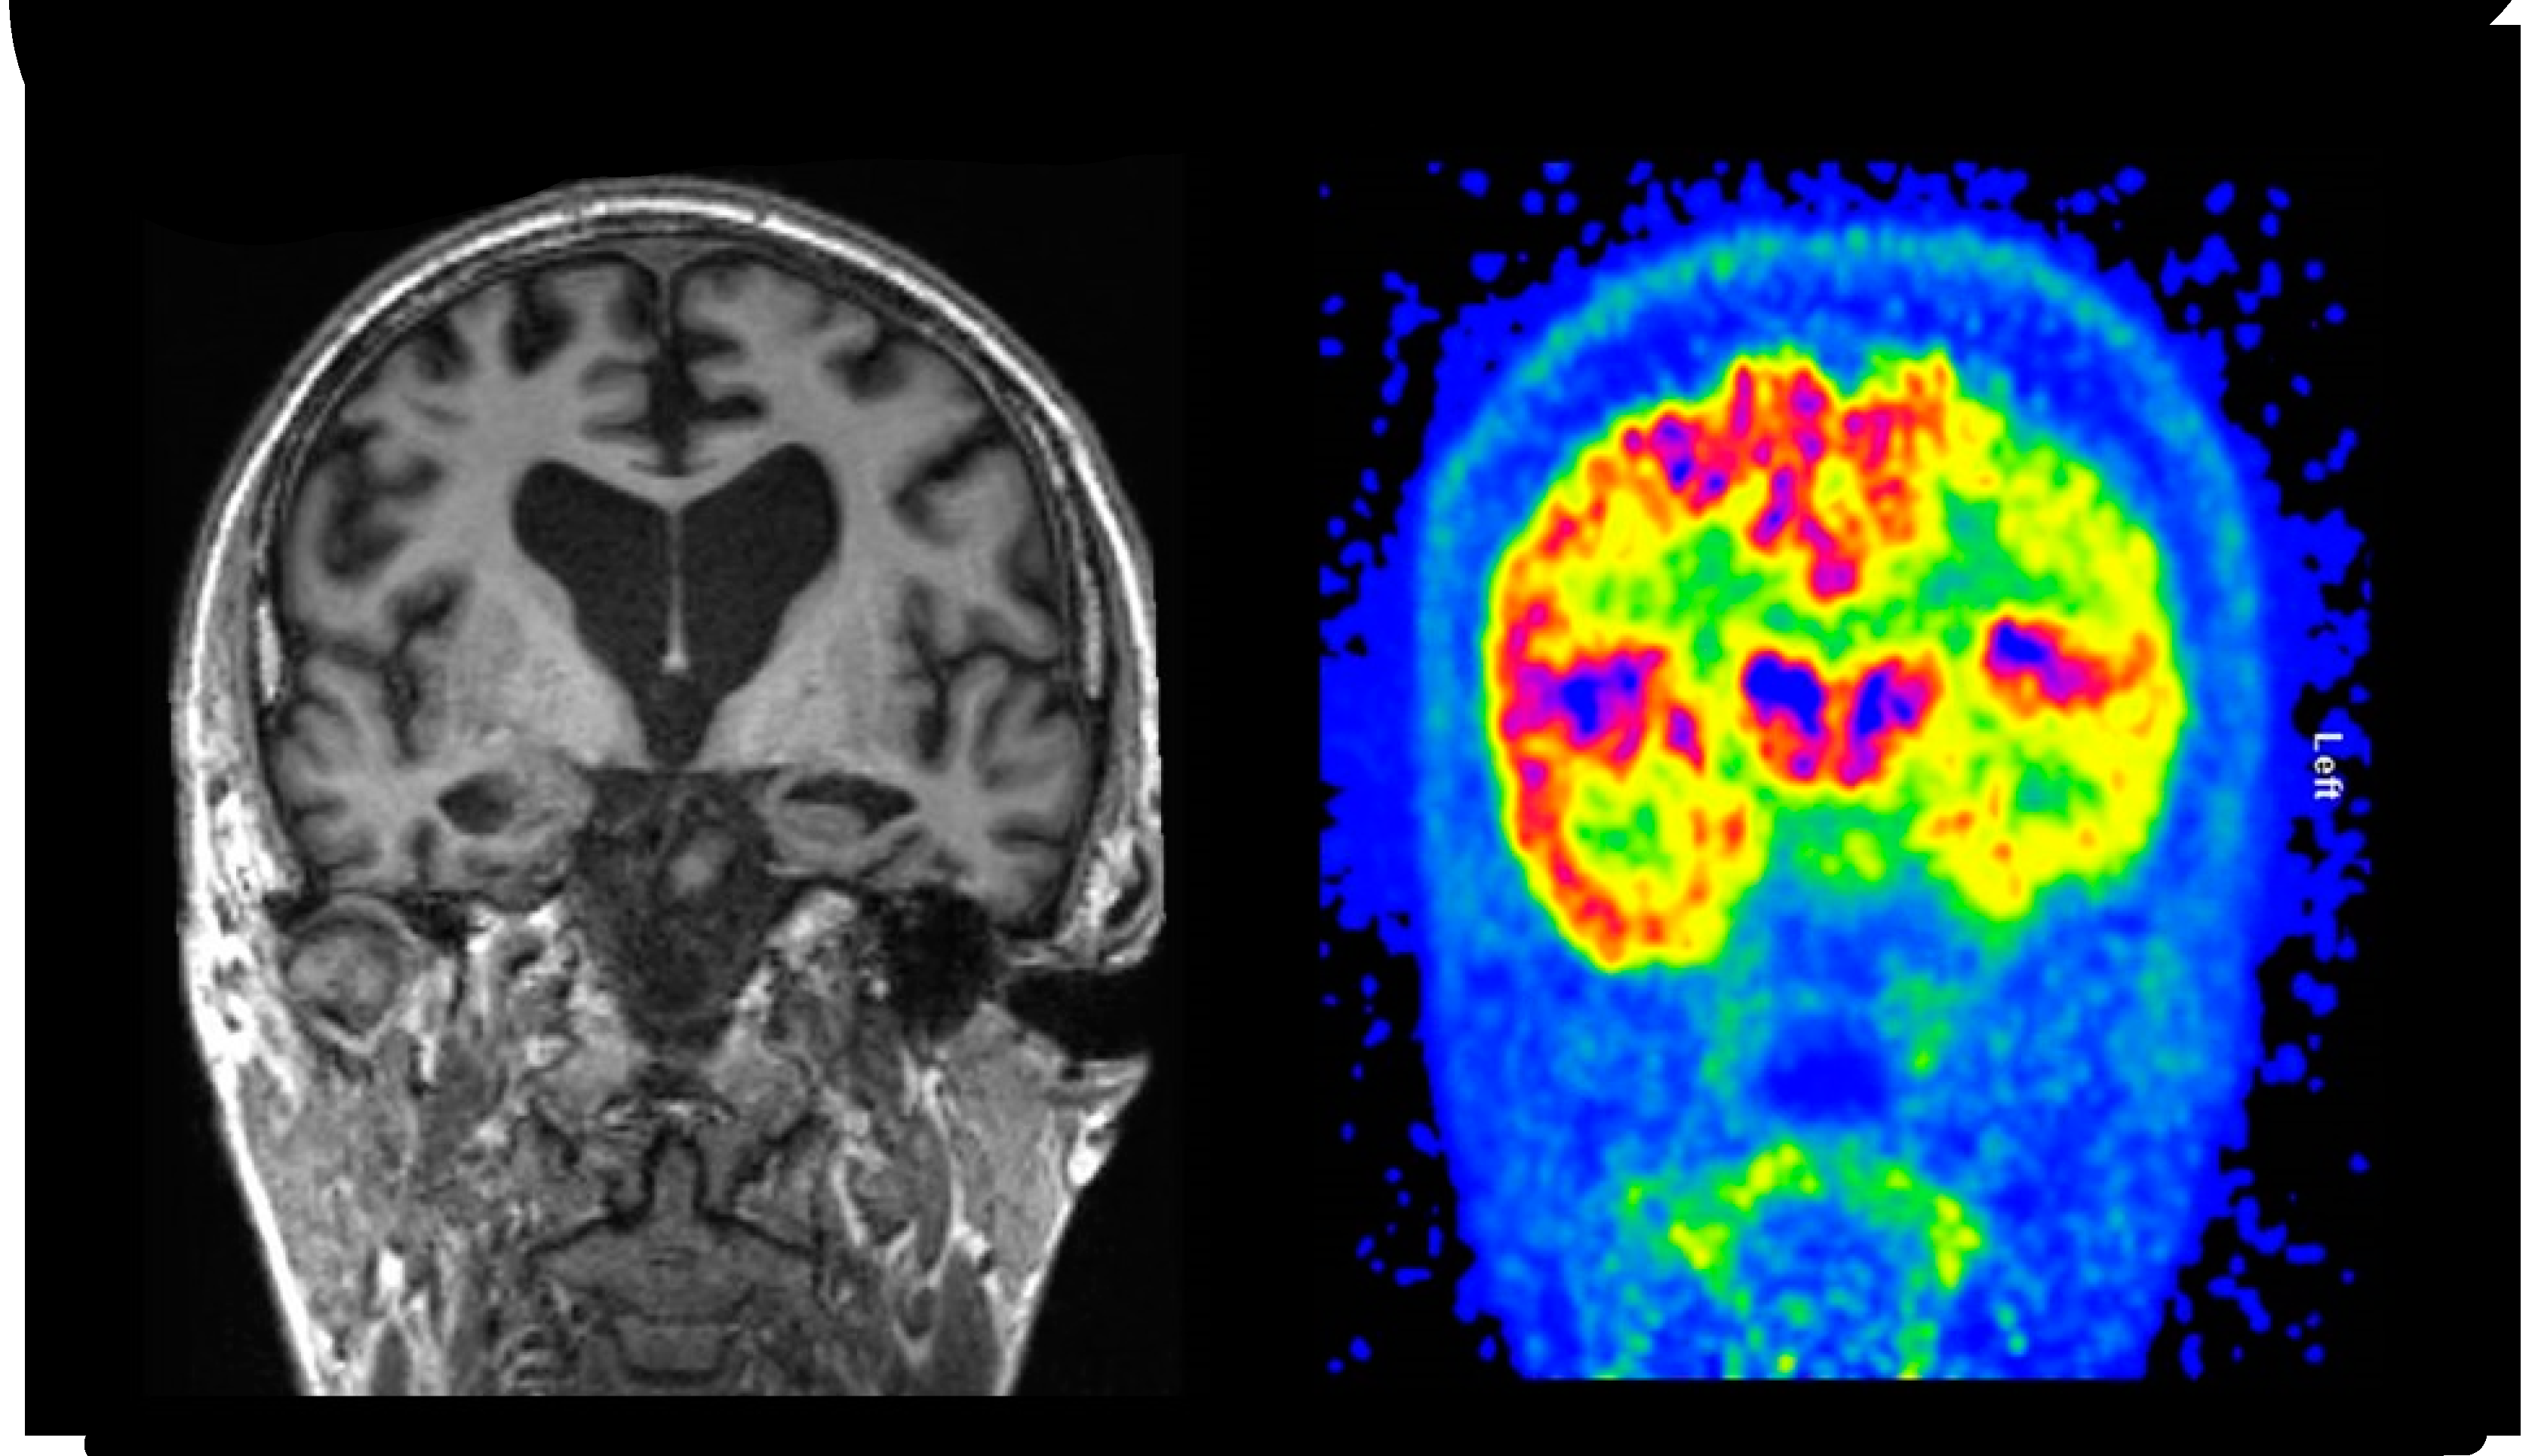
\includegraphics[
                    width=3.5cm,
                    trim={4cm 3cm 60cm 6cm},
                    clip
                ]{data/fdg_t1.png}
            };
            \node[label=below:{PET}] at (3, 0) {
                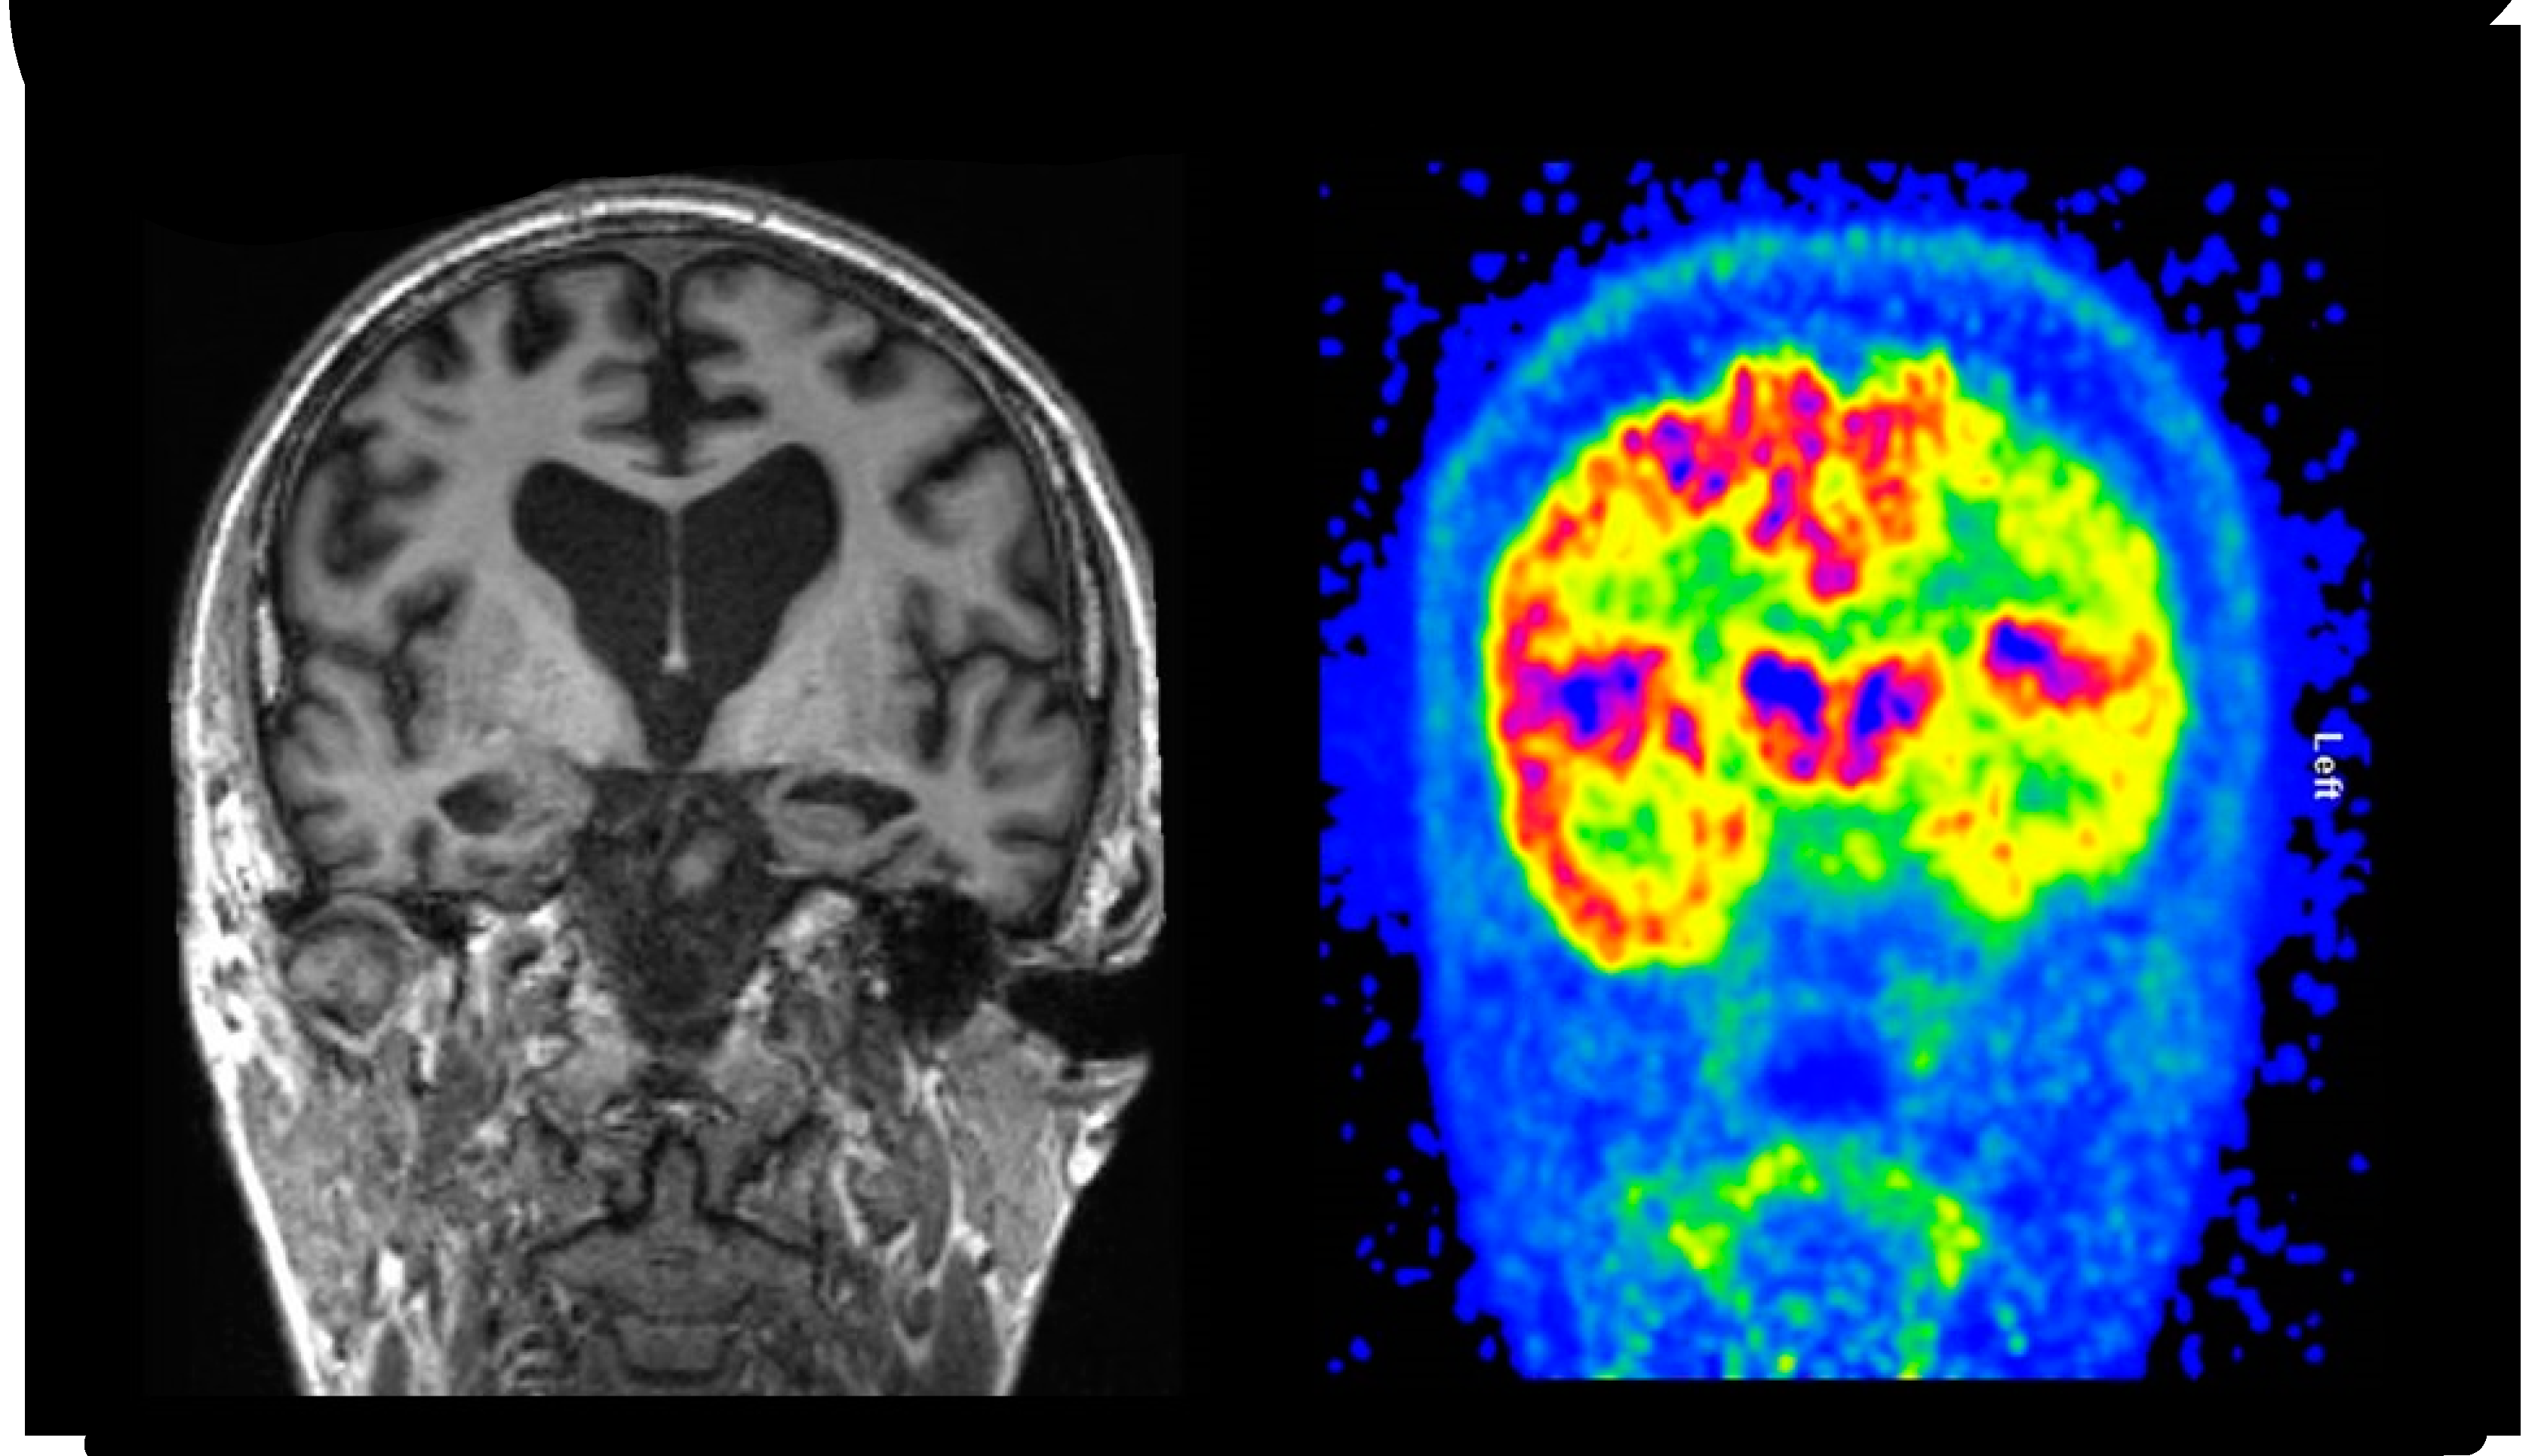
\includegraphics[
                    width=3.5cm,
                    trim={60cm 3cm 4cm 6cm},
                    clip
                ]{data/fdg_t1.png}
            };
        }
        \only<7>{
            \node[] at (-0.8, 0.5) {
                \dementia{2}
            };
        }
        \only<8>{
            \node[] at (-0.8, 0.5) {
                \dementia{3}
            };
        }
        \only<9>{
            \node[] at (-0.8, 0.5) {
                \dementia{4}
            };
        }
    \end{tikzpicture}
\end{frame}
    \newcommand{\neuron}[3]{
    \node[circle, draw=black, fill=#2] (#1) at #3 {};
}

\begin{frame}{Explainable artificial intelligence}
    \begin{tikzpicture}
        \node[] at (-5.25, -3.5) {};
        \node[] at (5.25, 3.5) {};

        \node[
            draw=black,
            fill=cyan!15,
            minimum height=3cm,
            minimum width=4.3cm,
            label=above:\footnotesize{\textbf{Artificial neural network}}
        ] (model) at (0, 0) {};

        \def\hsep{0.7}
        \def\vsep{0.5}
        \def\edgecolor{gray}
        \def\edgeopacity{0.5}
        \def\neuroncolour{gray}

        \only<1>{
            \neuron{n00}{\neuroncolour}{($ (model) + (-2 * \hsep, -2 * \vsep) $)}
            \neuron{n01}{\neuroncolour}{($ (model) + (-2 * \hsep, -\vsep) $)}
            \neuron{n02}{\neuroncolour}{($ (model) + (-2 * \hsep, 0) $)}
            \neuron{n03}{\neuroncolour}{($ (model) + (-2 * \hsep, \vsep) $)}
            \neuron{n04}{\neuroncolour}{($ (model) + (-2 * \hsep, 2 * \vsep) $)}

            \neuron{n10}{\neuroncolour}{($ (model) + (-\hsep, -1.5 * \vsep) $)}
            \neuron{n11}{\neuroncolour}{($ (model) + (-\hsep, -0.5 * \vsep) $)}
            \neuron{n12}{\neuroncolour}{($ (model) + (-\hsep, 0.5 * \vsep) $)}
            \neuron{n13}{\neuroncolour}{($ (model) + (-\hsep, 1.5 * \vsep) $)}

            \neuron{n20}{\neuroncolour}{($ (model) + (0, -\vsep) $)}
            \neuron{n21}{\neuroncolour}{(model)}
            \neuron{n22}{\neuroncolour}{($ (model) + (0, \vsep) $)}

            \neuron{n30}{\neuroncolour}{($ (model) + (\hsep, -0.5 * \vsep) $)}
            \neuron{n31}{\neuroncolour}{($ (model) + (\hsep, 0.5 * \vsep) $)}

            \neuron{n40}{\neuroncolour}{($ (model) + (2 * \hsep, 0) $)}

            \draw[-stealth, \edgecolor, opacity=\edgeopacity] (model.west) -- (n00);
            \draw[-stealth, \edgecolor, opacity=\edgeopacity] (model.west) -- (n01);
            \draw[-stealth, \edgecolor, opacity=\edgeopacity] (model.west) -- (n02);
            \draw[-stealth, \edgecolor, opacity=\edgeopacity] (model.west) -- (n03);
            \draw[-stealth, \edgecolor, opacity=\edgeopacity] (model.west) -- (n04);

            \foreach \i in {0,...,4} {
                \foreach \j in {0,...,3} {
                    \draw[\edgecolor, opacity=\edgeopacity] (n0\i) -- (n1\j);
                }
            }
            \foreach \i in {0,...,3} {
                \foreach \j in {0,...,2} {
                    \draw[\edgecolor, opacity=\edgeopacity] (n1\i) -- (n2\j);
                }
            }
            \foreach \i in {0,...,2} {
                \foreach \j in {0,...,1} {
                    \draw[\edgecolor, opacity=\edgeopacity] (n2\i) -- (n3\j);
                }
            }
            \foreach \i in {0,...,1} {
                \draw[\edgecolor, opacity=\edgeopacity] (n3\i) -- (n40);
            }

            \draw[-stealth, \edgecolor, opacity=\edgeopacity] (n40) -- (model.east);
        }
        \only<2>{
            \neuron{n00}{black!25}{($ (model) + (-2 * \hsep, -2 * \vsep) $)}
            \neuron{n01}{black!90}{($ (model) + (-2 * \hsep, -\vsep) $)}
            \neuron{n02}{black!72}{($ (model) + (-2 * \hsep, 0) $)}
            \neuron{n03}{black!99}{($ (model) + (-2 * \hsep, \vsep) $)}
            \neuron{n04}{black!10}{($ (model) + (-2 * \hsep, 2 * \vsep) $)}

            \neuron{n10}{black!55}{($ (model) + (-\hsep, -1.5 * \vsep) $)}
            \neuron{n11}{black!92}{($ (model) + (-\hsep, -0.5 * \vsep) $)}
            \neuron{n12}{black!31}{($ (model) + (-\hsep, 0.5 * \vsep) $)}
            \neuron{n13}{black!7}{($ (model) + (-\hsep, 1.5 * \vsep) $)}

            \neuron{n20}{black!50}{($ (model) + (0, -\vsep) $)}
            \neuron{n21}{black!10}{(model)}
            \neuron{n22}{black!100}{($ (model) + (0, \vsep) $)}

            \neuron{n30}{black!75}{($ (model) + (\hsep, -0.5 * \vsep) $)}
            \neuron{n31}{black!65}{($ (model) + (\hsep, 0.5 * \vsep) $)}

            \neuron{n40}{black!95}{($ (model) + (2 * \hsep, 0) $)}

            \draw[-stealth, \edgecolor, opacity=\edgeopacity] (model.west) -- (n00);
            \draw[-stealth, \edgecolor, opacity=\edgeopacity] (model.west) -- (n01);
            \draw[-stealth, \edgecolor, opacity=\edgeopacity] (model.west) -- (n02);
            \draw[-stealth, \edgecolor, opacity=\edgeopacity] (model.west) -- (n03);
            \draw[-stealth, \edgecolor, opacity=\edgeopacity] (model.west) -- (n04);

            \foreach \i in {0,...,4} {
                \foreach \j in {0,...,3} {
                    \draw[\edgecolor, opacity=\edgeopacity] (n0\i) -- (n1\j);
                }
            }
            \foreach \i in {0,...,3} {
                \foreach \j in {0,...,2} {
                    \draw[\edgecolor, opacity=\edgeopacity] (n1\i) -- (n2\j);
                }
            }
            \foreach \i in {0,...,2} {
                \foreach \j in {0,...,1} {
                    \draw[\edgecolor, opacity=\edgeopacity] (n2\i) -- (n3\j);
                }
            }
            \foreach \i in {0,...,1} {
                \draw[\edgecolor, opacity=\edgeopacity] (n3\i) -- (n40);
            }

            \draw[-stealth, \edgecolor, opacity=\edgeopacity] (n40) -- (model.east);

            \node[anchor=east, draw=black, inner sep=0pt] (input) at ($ (model.west) + (-0.77, 0) $) {
                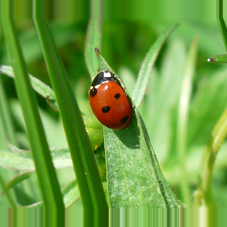
\includegraphics[width=2cm]{data/ladybug.png}
            };
            \cnnarrow{(input.east)}{(model.west)}{black}

            \node[anchor=west] (output) at ($ (model.east) + (0.77, 0) $) {
                Ladybug
            };
            \cnnarrow{(model.east)}{(output.west)}{black}

            \draw[-Latex, line width=3pt] ($ (model.south west) + (0.1, -0.4) $) -- ($ (model.south east) + (-0.1, -0.4) $);

            \node[] at (0, -2.3) {
                \textit{Forward pass}
            };
        }
        \only<3>{
            \neuron{n00}{red!25!black}{($ (model) + (-2 * \hsep, -2 * \vsep) $)}
            \neuron{n01}{red!90!black}{($ (model) + (-2 * \hsep, -\vsep) $)}
            \neuron{n02}{yellow!15!red}{($ (model) + (-2 * \hsep, 0) $)}
            \neuron{n03}{red!99!black}{($ (model) + (-2 * \hsep, \vsep) $)}
            \neuron{n04}{red!10!black}{($ (model) + (-2 * \hsep, 2 * \vsep) $)}

            \neuron{n10}{red!55!black}{($ (model) + (-\hsep, -1.5 * \vsep) $)}
            \neuron{n11}{yellow!20!red}{($ (model) + (-\hsep, -0.5 * \vsep) $)}
            \neuron{n12}{yellow!90!red}{($ (model) + (-\hsep, 0.5 * \vsep) $)}
            \neuron{n13}{red!7!black}{($ (model) + (-\hsep, 1.5 * \vsep) $)}

            \neuron{n20}{red!90!black}{($ (model) + (0, -\vsep) $)}
            \neuron{n21}{red!30!black}{(model)}
            \neuron{n22}{yellow!70!red}{($ (model) + (0, \vsep) $)}

            \neuron{n30}{yellow!40!red}{($ (model) + (\hsep, -0.5 * \vsep) $)}
            \neuron{n31}{red!65!black}{($ (model) + (\hsep, 0.5 * \vsep) $)}

            \neuron{n40}{red}{($ (model) + (2 * \hsep, 0) $)}

            \draw[stealth-, red, opacity=\edgeopacity] (model.west) -- (n00);
            \draw[stealth-, red, opacity=\edgeopacity] (model.west) -- (n01);
            \draw[stealth-, red, opacity=\edgeopacity] (model.west) -- (n02);
            \draw[stealth-, red, opacity=\edgeopacity] (model.west) -- (n03);
            \draw[stealth-, red, opacity=\edgeopacity] (model.west) -- (n04);

            \foreach \i in {0,...,4} {
                \foreach \j in {0,...,3} {
                    \draw[red, opacity=\edgeopacity] (n0\i) -- (n1\j);
                }
            }
            \foreach \i in {0,...,3} {
                \foreach \j in {0,...,2} {
                    \draw[red, opacity=\edgeopacity] (n1\i) -- (n2\j);
                }
            }
            \foreach \i in {0,...,2} {
                \foreach \j in {0,...,1} {
                    \draw[red, opacity=\edgeopacity] (n2\i) -- (n3\j);
                }
            }
            \foreach \i in {0,...,1} {
                \draw[red, opacity=\edgeopacity] (n3\i) -- (n40);
            }

            \draw[stealth-, red, opacity=\edgeopacity] (n40) -- (model.east);

            \node[anchor=east, draw=black, inner sep=0pt] (input) at ($ (model.west) + (-0.77, 0) $) {
                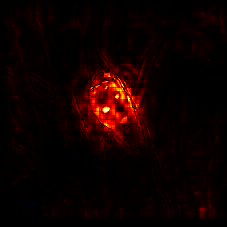
\includegraphics[width=2cm]{data/ladybug_explanation.png}
            };
            \lrparrow{(model.west)}{(input.east)}{red}

            \node[anchor=west, text=red] (output) at ($ (model.east) + (0.77, 0) $) {
                Ladybug
            };
            \lrparrow{(output.west)}{(model.east)}{red}

            \draw[Latex-, line width=3pt, red] ($ (model.south west) + (0.1, -0.4) $) -- ($ (model.south east) + (-0.1, -0.4) $);

            \node[text=red] at (0, -2.3) {
                \textit{Backward pass}
            };
        }
    \end{tikzpicture}
\end{frame}


\end{document}
